\subsection{Hamilton's Principle}
This assignment asks to get the equations of motion using the Hamilton Principle:
\begin{equation}
    \begin{split}
        \int_{t_1}^{t_2}\\delta (T-V+W)dt = 0
    \end{split}
\end{equation}

Using the theory discussed in the lecture we can split the term into different contributions::

% \begin{equation}
%     \begin{split}
%         \int_{t_1}^{t_2}\int_0^L \left[
%             \underbrace{\frac{\partial L}{\partial q} \\delta  q}_{A} + 
%             \underbrace{\frac{\partial L}{\partial q'}\\delta  q'}_{B} + 
%             \underbrace{\frac{\partial L}{\partial q''}\\delta  q''}_{C} + 
%             \underbrace{\frac{\partial L}{\partial \dot q} \\delta  \dot q}_{D} + 
%             \underbrace{\frac{\partial L}{\partial \dot q'} \\delta  \dot q'}_{E}+ 
%             \\delta  \text{W}\right]dxdt 
%     \end{split}
% \end{equation}
% \begin{equation}
%     \begin{split}
%         &\frac{\partial L}{\partial w} - \frac{\partial}{\partial x}\left(\frac
%         {\partial L}{w'}\right) + \frac{\partial ^2}{\partial x^2}\left(\frac
%         {\partial L}{\partial w''}\right) - \frac{\partial}{\partial t}\left(\frac{\partial L}{\partial \dot w}\right) + \frac{\partial }{\partial x}\left(\frac{\partial}{\partial t}\left(\frac{\partial L}{\partial \dot w'}\right)\right) + p(x,t) = 0\\
%         &x \in [0;L]
%     \end{split}
% \end{equation}

Remembering the result of the Hamilton principle from the lecture:

\begin{figure}[ht]
    \centering
    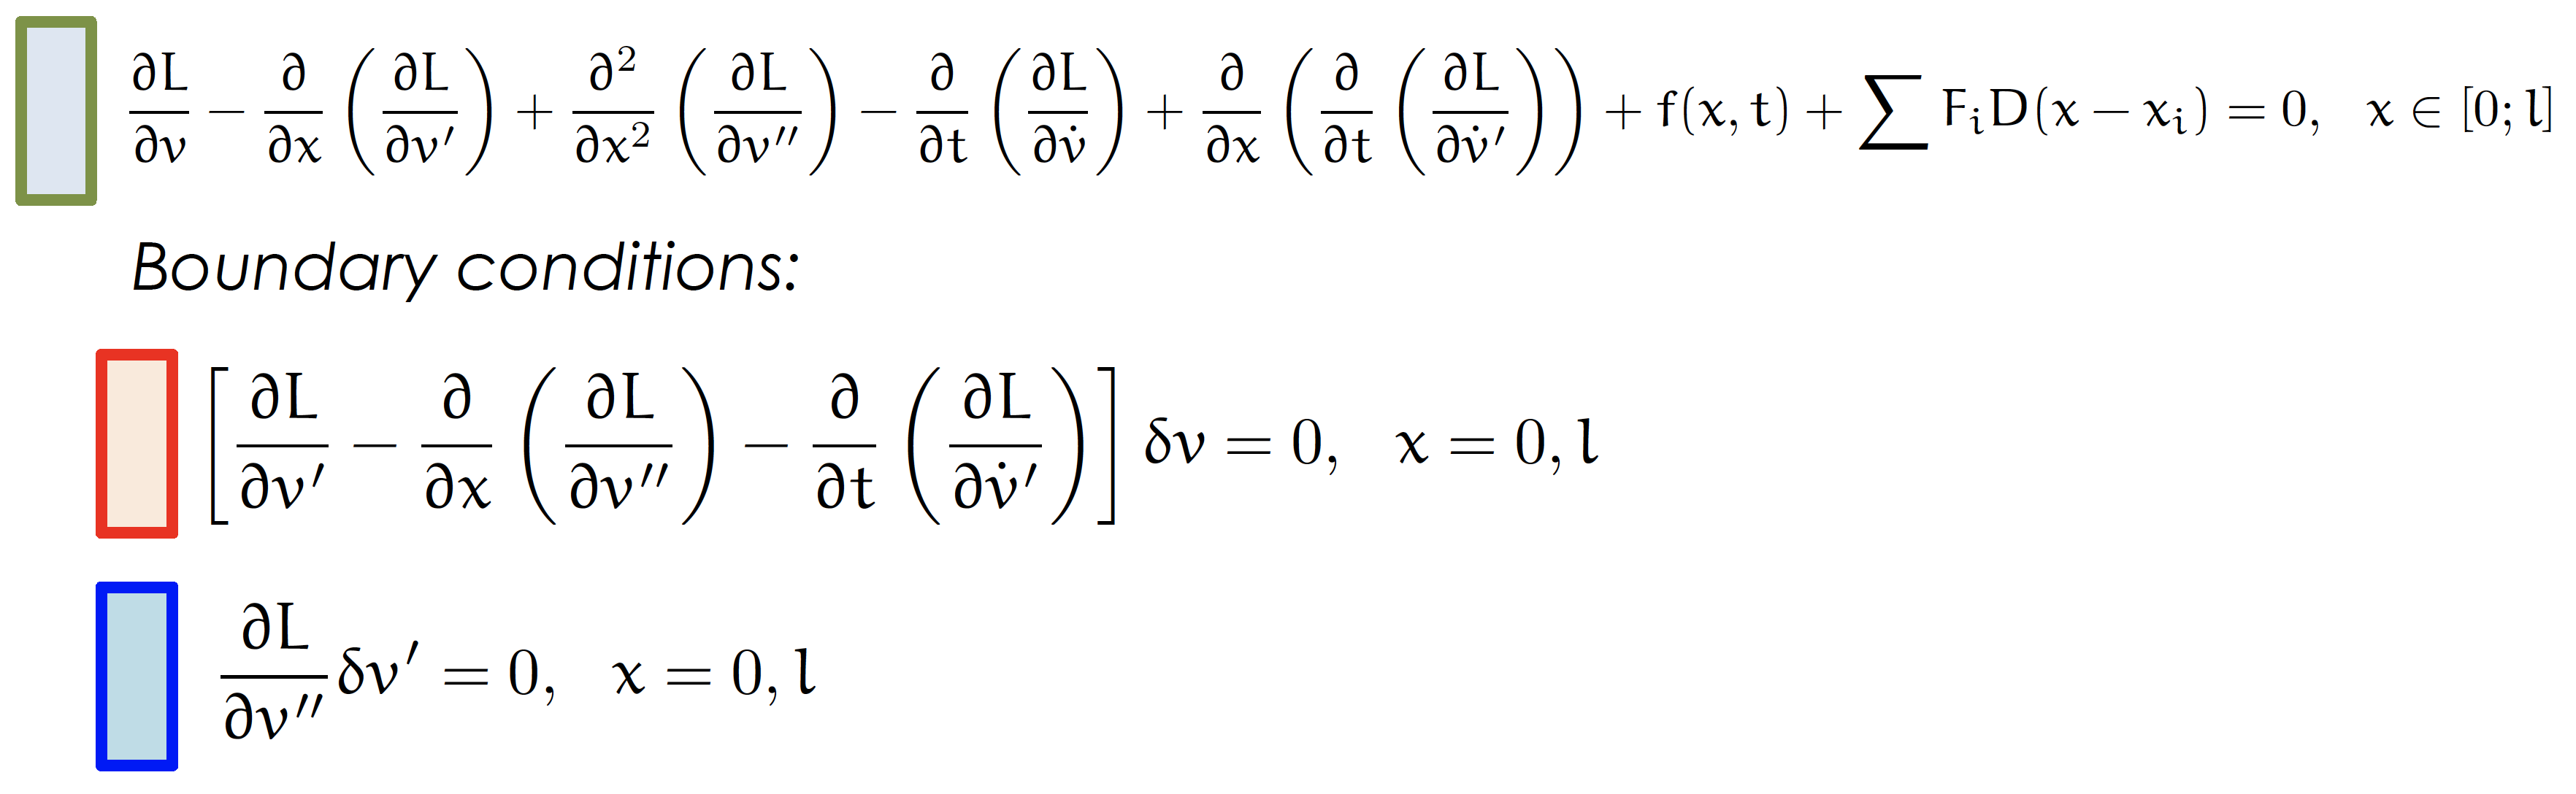
\includegraphics[scale=0.2]{images/Hamilton.png}
    \caption{Hamilton Formulas for a continuous system}
    %label always in the end
    \label{fig:hamilton}
\end{figure}

We consider w our variable instead of v.

\begin{equation}
    \begin{split}
        &\frac{\partial L}{\partial w} = 0
    \end{split}
\end{equation}

\begin{equation}
    \begin{split}
        \frac{\partial}{\partial x}\frac{\partial L}{\partial w'} = 0 
    \end{split}
\end{equation}

\begin{equation}
    \begin{split}
        &\frac{\partial^2}{\partial x^2}\frac{\partial L}{\partial w''} = -E\left(I(x)w^{(4)}+2I'(x)w^{(3)}+I'(x)'w''\right)
    \end{split}
\end{equation}

\begin{equation}
    \begin{split}
        \frac{\partial}{\partial t}\frac{\partial L}{\partial \dot w} = A(x)\rho \ddot w
    \end{split}
\end{equation}

\begin{equation}
    \begin{split}
        &\frac{\partial}{\partial x}\left(\frac{\partial}{\partial t}\left(\frac{\partial L}{\partial \dot w'}\right)\right) = \rho \left(I(x)\ddot w''+I'(x)\ddot w'\right)
    \end{split}
\end{equation}

\begin{equation}
    \begin{split}
        f(x,t) = p(x,t)
    \end{split}
\end{equation}

\begin{equation}
    \begin{split}
        \frac{\partial L }{\partial w'}= 0
    \end{split}
\end{equation}

\begin{equation}
    \begin{split}
        \frac{\partial}{\partial x}(\frac{\partial L}{\partial  w''}) = -E\left(I(x)w^{(3)}+I'(x)w''\right)
    \end{split}
\end{equation}

\begin{equation}
    \begin{split}
        \frac{\partial}{\partial t}(\frac{\partial L}{\partial \dot w'})= I(x)\rho \ddot w'
    \end{split}
\end{equation}

\subsubsection{Differential Equation aka green part}

Therefore the green part comes to:

\begin{equation}
    \begin{split}
        p(x,t)-E\left(I(x)w^{(4)}+2I'(x)w^{(3)}+I'(x)'w''\right)+\rho \left(I(x)\ddot w''+I'(x)\ddot w'\right)-A(x)\rho \ddot w = 0
    \end{split}
\end{equation}

\textbf{Comparing this solution to the Euler-Bernoulli Equation:}

\begin{equation}
    \begin{split}
        p(x,t) = EIw^{(4)} + A(x)\rho \ddot w
    \end{split}
\end{equation}

What we can see is that the additional terms from the green expression come from the derivative of I. This comes from the changing cross section and the thus changing moment of Inertia I. Secondly we had a term with $\dot w'$ in the kinetic energy arising through the change in thickness which is considered here. (not the case for the euler bernoulli beam).

\subsubsection{Boundary conditions with virtual displacement aka Red Part}

\begin{equation}
    \begin{split}
        \left[\vphantom{\int}\mathrm{\delta w(x)}\left(E\left(I(x)w^{(3)}+I'(x)w''\right)-I(x)\rho \ddot w'\right)\right]_0^L  = 0
    \end{split}
\end{equation}

\subsubsection{Blue part}

\begin{equation}
    \begin{split}
        \left[-\mathrm{\delta w'(x)}\vphantom{\int}EI(x)w''\right]_0^L = 0
    \end{split}
\end{equation}

\subsection{Analysis}

\begin{equation}
    \begin{split}
        I(0) = \frac{1}{12}h_0^3 \text{ and } I(L) = \frac{1}{12}h_L^3
    \end{split}
\end{equation}

as well as

\begin{equation}
    \begin{split}
        I'(0) = \frac{1}{4}h(0)^2*\frac{h_L - h_0}{L} = \frac{1}{4}h_0^2*\frac{h_L - h_0}{L}
    \end{split}
\end{equation}

and

\begin{equation}
    \begin{split}
        I'(L) = \frac{1}{4}h_L^2*\frac{h_L - h_0}{L}
    \end{split}
\end{equation}

Beginning with the blue part and pluggin in the boundary values:

\begin{equation}
    \begin{split}
        -\mathrm{\delta w'(L)}\vphantom{\int}E\text{h}_L^3w''(L) + \mathrm{\delta w'(0)}\vphantom{\int}E\text{h}_0^3w''(0) = 0
    \end{split}
\end{equation}

As we have a clamped end (w, $\delta$w and their first three derivatives are 0) and a supported end (w, $\delta$w and their first derivative is 0) we arrive at:

\begin{equation}
    \begin{split}
        0 = 0
    \end{split}
\end{equation}

For the red part:

\begin{equation}
    \begin{split}
        &\delta w(L) \left(E\left(I(L)w^{(3)}(L) + I'(L)w''(L)\right) - I(L)\rho \ddot w'(L)\right) - \\
        &\delta w(0) \left(E\left(I(0)w^{(3)}(0) + I'(0)w''(0)\right) - I(0)\rho \ddot w'(0)\right) = 0
    \end{split}
\end{equation}

Note that both $\delta w(0) = \delta w(L) = 0$. The coefficients
\begin{center}
    $E\left(I(L)w^{(3)}(L) + I'(L)w''(L)\right) - I(L)\rho \ddot w'(L)$
\end{center}
 
and 

\begin{center}
    $E\left(I(0)w^{(3)}(0) + I'(0)w''(0)\right) - I(0)\rho \ddot w'(0)$
\end{center}

represent the forces at the boundaries. To determine these forces we would have to solve the differential equation to get a solution for w which we can use to get the forces.

\subsection{Analysis with open second end}

Nothing changes in the application of the Hamilton Principle. However when analysing the boundaries we see some changes:\\
\vspace{5mm}
\noindent Starting again with the blue:

\begin{equation}
    \begin{split}
        -\mathrm{\delta w'(L)}E\text{h}_L^3w''(L) + \mathrm{\delta w'(0)}\vphantom{\int}E\text{h}_0^3w''(0) = 0
    \end{split}
\end{equation}

As before the w terms at $x = 0$ vanish. However now $\delta w'(L) \neq 0$ thus we get 

\begin{equation}
    \begin{split}
        E\text{h}_L^3w''(L) = 0
    \end{split}
\end{equation}

So the slope at the vertical displacement of the free end has to stay constant.\\
\vspace{5mm}
\noindent For the red part we get:

\begin{equation}
    \begin{split}
        &\delta w(L) \left(E\left(I(L)w^{(3)}(L) + I'(L)w''(L)\right) - I(L)\rho \ddot w'(L)\right) - \\
        &\delta w(0) \left(E\left(I(0)w^{(3)}(0) + I'(0)w''(0)\right) - I(0)\rho \ddot w'(0)\right) = 0
    \end{split}
\end{equation}

As before $\delta w(0) = 0$ and the force of the boundary constraint is:

\begin{equation}
    \begin{split}
        E\left(I(0)w^{(3)}(0) + I'(0)w''(0)\right) - I(0)\rho \ddot w'(0)
    \end{split}
\end{equation}

However for the second end we have $\delta w(L) \neq 0$ which leads to:

\begin{equation}
    \begin{split}
        E\left(I(L)w^{(3)}(L) + I'(L)w''(L)\right) - I(L)\rho \ddot w'(L) = 0
    \end{split}
\end{equation}

Pluggin in the values for I and I':

\begin{equation}
    \begin{split}
        E\left(h_Lw^{(3)}(L) + 3*\frac{h_L - h_0}{L}w''(L)\right) - h_L\rho \ddot w'(L) = 0
    \end{split}
\end{equation}






